\documentclass[tikz,border=4mm]{standalone}
      \usepackage{tikz}
      \usetikzlibrary{arrows.meta,positioning,calc,shapes.geometric}
      \begin{document}
      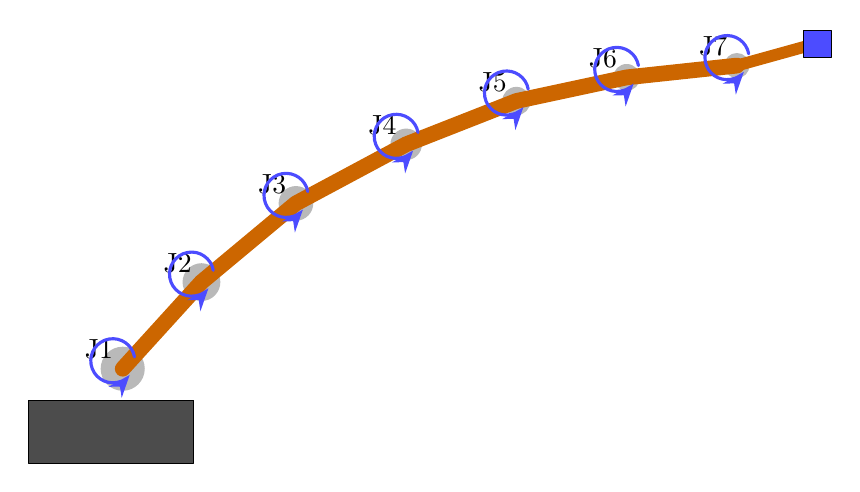
\begin{tikzpicture}[>=Stealth, line cap=round, line join=round]

\draw[fill=black!70] (1.0,1.3) rectangle (3.1,2.1);
\fill[fill=gray!55] (2.2,2.5) circle (0.28);
\fill[fill=gray!55] (3.2,3.6) circle (0.24);
\fill[fill=gray!55] (4.4,4.6) circle (0.22);
\fill[fill=gray!55] (5.8,5.35) circle (0.2);
\fill[fill=gray!55] (7.2,5.9) circle (0.18);
\fill[fill=gray!55] (8.6,6.2) circle (0.17);
\fill[fill=gray!55] (10.0,6.35) circle (0.16);
\draw[line width=0.2cm, orange!80!black] (2.2,2.5) -- (3.2,3.6) -- (4.4,4.6) -- (5.8,5.35) -- (7.2,5.9) -- (8.6,6.2) -- (10.0,6.35);
\draw[line width=0.15cm, orange!80!black] (10.0,6.35) -- (10.9,6.6);
\draw[fill=blue!70] (10.85,6.45) rectangle (11.2,6.8);
\foreach \x/\y/\label in {2.2/2.5/J1,3.2/3.6/J2,4.4/4.6/J3,5.8/5.35/J4,7.2/5.9/J5,8.6/6.2/J6,10.0/6.35/J7}{
  \node[above left] at (\x,\y) {\label};
  \draw[->, blue!70, line width=0.04cm] (\x+0.15,\y+0.15) arc[start angle=10,end angle=320,radius=0.28];
}

      \end{tikzpicture}
      \end{document}
